\subsection{Captura 1 - Empresa S.I.S.A.}

La primer red en la que realizamos una captura fue la correspondiente a la empresa S.I.S.A.
Esta es una red Wifi de uso exclusivo para los dispositivos personales \textit{(celulares, notebooks, tablets, etc)} de los empleados.
La captura tuvo lugar alrededor del mediodía, durante treinta minutos, lográndose capturar $6800$ paquetes, de los cuales $230$ pertenecen al protocolo ARP.

\begin{figure}[H]
  \centering
    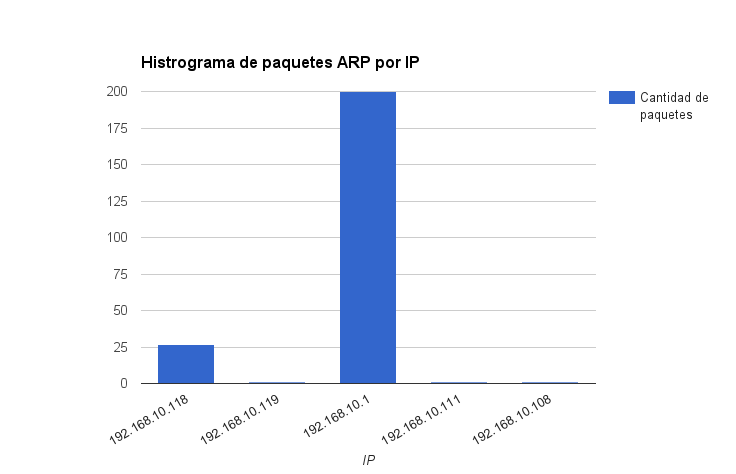
\includegraphics[width=1.1\textwidth]{imagenes/sisa/histograma.png}
  \caption{Histograma de los símbolos de la fuente $S_1$ (\textit{dirección IP de origen})}
  \label{fig:ejemplo}
\end{figure}

Esta red es privada y podemos ver que cuenta con pocos nodos, sólo 5 IPs. El tráfico ARP parece estar concentrado por la dirección \textit{192.168.10.1}.
Intuimos que la misma puede corresponder al router intentando resolver nuevas direcciones.

\begin{figure}[H]
  \centering
    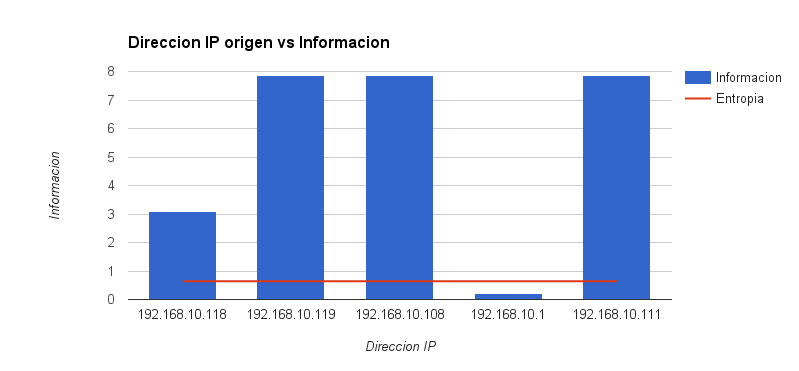
\includegraphics[width=1.1\textwidth]{imagenes/sisa/ip_informacion.png}
  \caption{Información de los símbolos de la fuente $S_1$ (\textit{dirección IP de origen})}
  \label{fig:ejemplo}
\end{figure}

Como habíamos anticipado al explicar la función de los distintos gráficos existe una fuerte correlación entre este gráfico y el anterior. Se puede apreciar
claramente que los nodos con mayor frecuencia son a su vez los que menos información proveen. Asimismo el nodo que resultó distinguido en el anterior gráfico por
presentar la mayor frecuencia, en éste queda distinguido por ser el único con una información menor a la entropía de la fuente.

\begin{figure}[H]
  \centering
    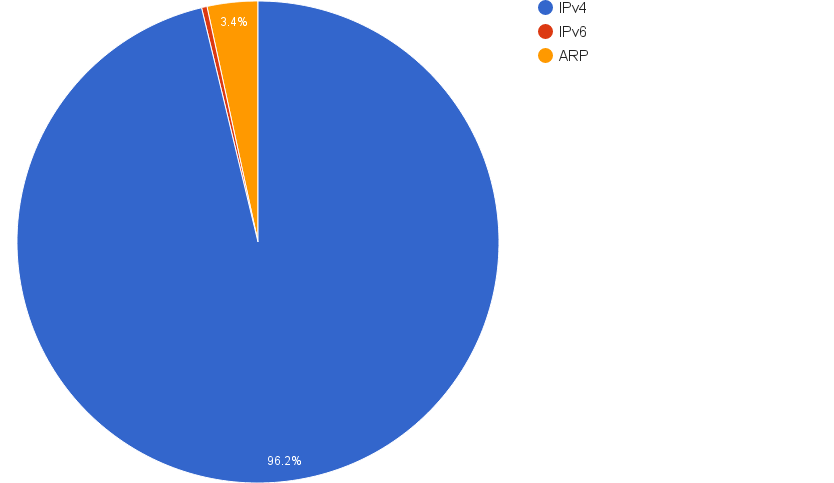
\includegraphics[width=0.7\textwidth]{imagenes/sisa/proporcion_protocolos.png}
  \caption{Proporción de protocolos observados en el trafico de la red S.I.S.A.}
  \label{fig:ejemplo}
\end{figure}

Se puede ver claramente la predominancia del protocolo \textit{IPv4} en esta red y además, podemos ver que el overhead impuesto por el protocolo ARP es de tan solo un 3.4\% del tráfico total.

\begin{figure}[H]
  \centering
    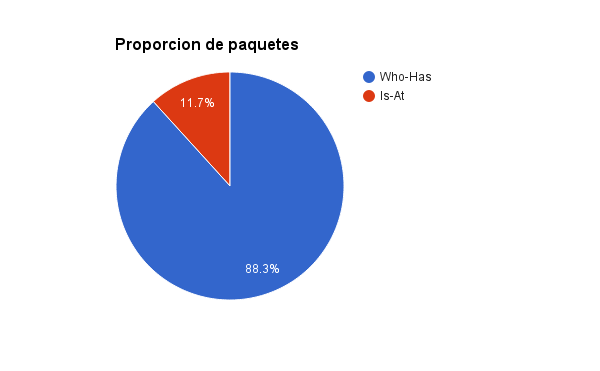
\includegraphics[width=0.9\textwidth]{imagenes/sisa/proporcion_paquetes_arp.png}
  \caption{Proporción de paquetes who-has e is-at en red S.I.S.A.}
  \label{fig:ejemplo}
\end{figure}

De todo del tráfico ARP capturado en la red S.I.S.A, casi un 90\% corresponde a paquetes \textit{who-has}. Esta proporción no sorprende, ya que probablemente el router de la red este administrando las IPs disponibles \textit{(DHCP\footnote{DHCP: \url{http://en.wikipedia.org/wiki/Dynamic_Host_Configuration_Protocol}})} y utilice el protocolo ARP para para mantener actualizado su listado de IPs disponibles \textit{(no asignadas a un host)}.


%La red cuenta con 5 nodos, uno de los cuales actúa como router. Nosotros esperábamos que la gran mayoría de los paquetes \textit{who-has} que enviara el router iban a a ser broadcast y por lo tanto lo iban a recibir los otros 4 nodos. De éstos 4 nodos que recibían el \textit{who-has} uno de ellos respondería con un \textit{is-at}, lo cual resultaría en una proporción aproximada de $80\%$ de \textit{who-has} y $20\%$ de \textit{is-at} (1 por cada 4). Creemos que la mayor cantidad de de paquetes \textit{who-has} puede deberse a que algunos \textit{who-has} no obtuvieron respuesta o que los dispositivos conectados a la red fueron cambiando pero recibieron las mismas IPs.

\begin{figure}[H]
  \centering
    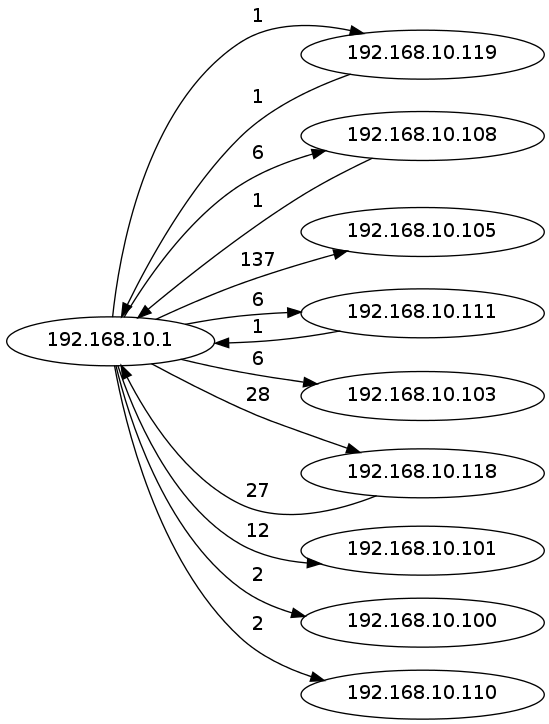
\includegraphics[width=0.6\textwidth]{imagenes/sisa/digrafo_sisa.png}
  \caption{Trafico de paquetes ARP entre las IP de la red S.I.S.A.}
  \label{fig:ejemplo}
\end{figure}

En este digrafo se puede ver claramente que la IP 192.168.10.1 corresponde al router, ya que concentra todo el tráfico de los otros host. Resulta curioso ver la insistencia del router al enviarle $137$ paquetes ARP a una misma IP, en comparación con las otras IPs, las cuales reciben a lo sumo $30$ paquetes ARP. No encontramos razones para esta disparidad.

\newpage